\documentclass[12pt]{article}
\usepackage{url}
\usepackage{bm}
\usepackage{bbm}
\usepackage{amsmath,amsfonts,amssymb,amsthm,rotating,dsfont}
\usepackage{algorithm}
\usepackage{pdflscape}
\usepackage{enumerate}
\usepackage{xcolor}
\usepackage{multirow}
\usepackage[left = 1 in, right = 1 in, top = 1 in, bottom = 1 in]{geometry}
\usepackage{setspace}
\usepackage{lineno}
\usepackage{threeparttable}
\usepackage{xr}
\usepackage{adjustbox}
\usepackage{graphicx}
\usepackage{tabularx,booktabs}
\usepackage{hyperref}

\newcommand{\tablesdir}{tables}

\begin{document}

\setcounter{table}{3}

 \clearpage
 \setcounter{table}{2}
 \begin{table}[!htbp]
 \caption{\sc Downside Risk Factor Screening}\label{tbl:screening:variables}
 \begin{center}
 \begin{footnotesize}
 \newcolumntype{C}{>{\centering\arraybackslash}p{0.5cm}} 
\begin{tabular}{llCCCC}
\cmidrule(l){3-6} 
\multicolumn{2}{c}{} & \multicolumn{4}{c}{Horizon} \\ 
\cmidrule{1-2} \cmidrule(l){3-6} 
Model & Class & 1 & 3 & 6 & 12\\ 
\cmidrule{1-2} \cmidrule(l){3-6} 
MUNC & Macro & 80.8 & 82.5 & 76.7 & 70.0 \\ 
PCF1 & Stat & 70.0 & 66.7 & 57.5 & 47.5 \\ 
FUNC & Fin & 62.5 & 65.0 & 60.8 & 50.0 \\ 
QF1 & Stat & 70.0 & 52.5 & 45.0 & 25.0 \\ 
NFCI & Fin & 43.3 & 49.2 & 52.5 & 45.8 \\ 
PC1 & Stat & 50.8 & 58.3 & 48.3 & 32.5 \\ 
VIX & Fin & 58.3 & 53.3 & 45.0 & 33.3 \\ 
CISS & Fin & 50.0 & 48.3 & 43.3 & 19.2 \\ 
EBP & Fin & 35.8 & 43.3 & 38.3 & 35.8 \\ 
EPU & Text & 35.0 & 32.5 & 23.3 & 14.2 \\ 
CTG & Macro & 25.8 & 19.2 & 22.5 & 28.3 \\ 
RISK & Text & 20.8 & 29.2 & 10.0 & 6.7 \\ 
HPI & Macro & 10.8 & 23.3 & 19.2 & 12.5 \\ 
PRISK & Text & 16.7 & 18.3 & 8.3 & 18.3 \\ 
NPRISK & Text & 16.7 & 14.2 & 10.0 & 11.7 \\ 
WUI & Text & 18.3 & 18.3 & 8.3 & 6.7 \\ 
GPR & Text & 4.2 & 0.8 & 6.7 & 10.0 \\ 
\cmidrule(l){1-6} 
\end{tabular} 

 \end{footnotesize}
 \end{center}

  {\hspace{1em} \footnotesize This table reports the results of the downside risk factor screening exercise. For each predictor, the table lists the percentage of macroeconomic variables for which the coefficient on the predictor is statistically significant at the 5\% level. The percentages are obtained from quantile regression, with $p=0.05$, at horizons of 1, 3, 6, and 12 months. Significance is assessed on the basis of bootstrap standard errors. Predictors are sorted in descending order according to the average percentage of significant coefficients across horizons.
  }

 \end{table}

\clearpage
\begin{table}[!htbp]
	\caption{\sc Downside Risk Model Screening}\label{tbl:screening:models}
	\begin{center}
		\begin{tiny}
			\newcolumntype{C}{>{\centering\arraybackslash}p{0.6cm}} 
\begin{tabular}{lllCCCC} 
\cmidrule{1-7} 
\multicolumn{3}{c}{FRED-MD} & \multicolumn{4}{c}{$\overline{TLG}$} \\ 
\cmidrule{1-3} \cmidrule(l){4-7}
{$h$} & {Class} & {Model} & {QR} & {LR} & {SR} & {LSR} \\ 
\cmidrule{1-3} \cmidrule(l){4-7}
\multirow{16}{*}{1} & \multirow{2}{*}{Bench} & HIST & 0.0 & 0.0 & 0.0 & 0.0 \\ 
& & AR & 14.6 & 22.6 & 22.6 & 22.6\\ [1.5mm] 
& \multirow{5}{*}{Fin} & NFCI & 16.9 & 22.6 & 23.0 & 23.1 \\ 
& & EBP & 16.3 & 22.4 & 22.6 & 22.7 \\ 
& & FUNC & 18.2 & 23.3 & 24.2 & 24.2 \\ 
& & VIX & 17.2 & 22.9 & 23.2 & 23.2 \\ 
& & CISS & 19.1 & 23.7 & 24.2 & 24.2\\ [1.5mm] 
& \multirow{3}{*}{Macro} & MUNC & 20.9 & 23.1 & 25.2 & \textbf{25.4} \\ 
& & HPI & 15.8 & 23.1 & 22.9 & 23.0 \\ 
& & CTG & 15.6 & 22.6 & 22.7 & 22.7\\ [1.5mm] 
& \multirow{3}{*}{} & PC1 & 17.3 & 23.5 & 23.1 & 23.9 \\ 
& & QF1 & 19.1 & 23.1 & 23.7 & 23.9 \\ 
& & PCF1 & 20.6 & 23.7 & 25.0 & 25.0\\ [1.5mm] 
& \multirow{3}{*}{} & WUI & 15.5 & 22.6 & 22.7 & 22.7 \\ 
& & GPR & 14.8 & 22.6 & 22.6 & 22.7 \\ 
& & EPU & 16.7 & 22.7 & 23.1 & 23.1 \\ 
\cmidrule{1-3} \cmidrule(l){4-7}
\multirow{16}{*}{3} & \multirow{2}{*}{Bench} & HIST & 0.0 & 0.0 & 0.0 & 0.0 \\ 
& & AR & 16.2 & 22.1 & 22.1 & 22.1\\ [1.5mm] 
& \multirow{5}{*}{Fin} & NFCI & 20.7 & 22.7 & 23.1 & 24.0 \\ 
& & EBP & 18.9 & 21.7 & 21.5 & 22.2 \\ 
& & FUNC & 23.2 & 24.2 & 26.3 & 27.2 \\ 
& & VIX & 20.7 & 23.2 & 23.7 & 24.0 \\ 
& & CISS & 21.6 & 24.0 & 23.9 & 24.6\\ [1.5mm] 
& \multirow{3}{*}{Macro} & MUNC & 26.1 & 23.5 & 26.8 & \textbf{27.6} \\ 
& & HPI & 18.2 & 22.9 & 22.7 & 23.1 \\ 
& & CTG & 17.6 & 22.2 & 22.3 & 22.4\\ [1.5mm] 
& \multirow{3}{*}{} & PC1 & 20.5 & 24.1 & 23.4 & 25.0 \\ 
& & QF1 & 22.3 & 23.1 & 24.5 & 24.8 \\ 
& & PCF1 & 24.5 & 24.3 & 25.3 & 25.9\\ [1.5mm] 
& \multirow{3}{*}{} & WUI & 17.9 & 22.3 & 22.9 & 23.0 \\ 
& & GPR & 16.6 & 22.2 & 22.1 & 22.3 \\ 
& & EPU & 19.0 & 22.3 & 22.7 & 22.8 \\ 
\cmidrule{1-3} \cmidrule(l){4-7}
\multirow{16}{*}{6} & \multirow{2}{*}{Bench} & HIST & 0.0 & 0.0 & 0.0 & 0.0 \\ 
& & AR & 15.3 & 19.2 & 19.2 & 19.2\\ [1.5mm] 
& \multirow{5}{*}{Fin} & NFCI & 21.8 & 21.3 & 22.0 & 23.7 \\ 
& & EBP & 19.5 & 20.0 & 20.2 & 21.7 \\ 
& & FUNC & 24.0 & 22.4 & 24.9 & 25.9 \\ 
& & VIX & 20.2 & 20.7 & 21.4 & 21.9 \\ 
& & CISS & 22.0 & 22.2 & 22.0 & 23.0\\ [1.5mm] 
& \multirow{3}{*}{Macro} & MUNC & \textbf{26.4} & 21.3 & 24.2 & 25.1 \\ 
& & HPI & 19.0 & 21.4 & 21.0 & 21.6 \\ 
& & CTG & 17.6 & 19.5 & 20.0 & 20.2\\ [1.5mm] 
& \multirow{3}{*}{} & PC1 & 19.8 & 21.6 & 21.5 & 23.3 \\ 
& & QF1 & 20.6 & 20.3 & 21.5 & 21.9 \\ 
& & PCF1 & 25.6 & 23.1 & 24.6 & 25.3\\ [1.5mm] 
& \multirow{3}{*}{} & WUI & 17.2 & 19.4 & 19.7 & 20.2 \\ 
& & GPR & 15.7 & 19.2 & 19.2 & 19.4 \\ 
& & EPU & 18.0 & 19.5 & 19.2 & 19.4 \\ 
\cmidrule{1-3} \cmidrule(l){4-7}
\multirow{16}{*}{12} & \multirow{2}{*}{Bench} & HIST & 0.0 & 0.0 & 0.0 & 0.0 \\ 
& & AR & 11.1 & 14.7 & 14.7 & 14.7\\ [1.5mm] 
& \multirow{5}{*}{Fin} & NFCI & 16.0 & 15.8 & 15.5 & 17.2 \\ 
& & EBP & 14.7 & 16.4 & 15.7 & 17.6 \\ 
& & FUNC & 18.3 & 17.7 & 17.9 & 20.4 \\ 
& & VIX & 15.2 & 16.0 & 16.4 & 16.8 \\ 
& & CISS & 17.4 & 18.0 & 18.6 & 19.1\\ [1.5mm] 
& \multirow{3}{*}{Macro} & MUNC & \textbf{21.6} & 16.6 & 17.1 & 19.2 \\ 
& & HPI & 14.9 & 17.7 & 17.1 & 18.4 \\ 
& & CTG & 15.1 & 15.9 & 16.8 & 17.6\\ [1.5mm] 
& \multirow{3}{*}{} & PC1 & 14.3 & 16.3 & 16.0 & 17.4 \\ 
& & QF1 & 14.5 & 15.3 & 15.5 & 15.8 \\ 
& & PCF1 & 21.2 & 19.1 & 19.5 & 21.0\\ [1.5mm] 
& \multirow{3}{*}{} & WUI & 13.4 & 15.3 & 15.3 & 16.1 \\ 
& & GPR & 11.9 & 14.8 & 15.2 & 15.4 \\ 
& & EPU & 14.1 & 15.2 & 14.9 & 14.9 \\ 
\cmidrule{1-3} \cmidrule(l){4-7}
\end{tabular}

		\end{tiny}
	\end{center}

	{\hspace{1em} \footnotesize This table reports the results of the downside risk model screening exercise. For each downside risk factor and forecast horizon, the table lists the average tick loss gain associated with quantile regression, with $p=0.05$, and the three variants of the location-scale regression at horizons of 1, 3, 6, and 12 months. The gains are computed relative to the historical quantile benchmark. Bold values indicate the best-performing specification at each horizon in terms of the average tick loss gain.
	}

\end{table}

\clearpage
\begin{table}[!htbp]
\caption{\sc Model Confidence Set}\label{tbl:mcs}
\begin{center}
\begin{footnotesize}
\newcolumntype{C}{>{\centering\arraybackslash}p{0.6cm}} 
\begin{tabular}{lCCCCCCCC} 
\cmidrule{2-9} 
 & \multicolumn{8}{c}{Horizon} \\ 
\cmidrule{2-9} 
 & \multicolumn{2}{c}{1} & \multicolumn{2}{c}{3} & \multicolumn{2}{c}{6} & \multicolumn{2}{c}{12} \\ 
\cmidrule{2-3} \cmidrule(l){4-5} \cmidrule(l){6-7} \cmidrule(l){8-9} 
 & $\%$ & TLG & $\%$ & TLG & $\%$ & TLG & $\%$ & TLG\\ 
\cmidrule{1-1} \cmidrule(l){2-3} \cmidrule(l){4-5} \cmidrule(l){6-7} \cmidrule(l){8-9} 
All & 38.5 & 26.9 & 49.1 & 29.0 & 70.0 & 27.9 & 59.7 & 19.4 \\ 
\cmidrule{1-1} \cmidrule(l){2-3} \cmidrule(l){4-5} \cmidrule(l){6-7} \cmidrule(l){8-9} 
QR & 0.0 & 22.1 & 0.7 & 24.5 & 46.1 & 24.9 & 42.6 & 17.6 \\ 
LSR & 77.3 & 26.9 & 97.9 & 29.0 & 94.3 & 27.9 & 77.3 & 19.4 \\ 
\cmidrule{1-1} \cmidrule(l){2-3} \cmidrule(l){4-5} \cmidrule(l){6-7} \cmidrule(l){8-9} 
1 Factor & 42.9 & 26.6 & 50.0 & 28.7 & 60.7 & 27.9 & 71.4 & 19.4 \\ 
2 Factors & 43.6 & 26.9 & 51.3 & 29.0 & 79.5 & 27.1 & 70.5 & 18.3 \\ 
3 Factors & 35.6 & 26.9 & 48.3 & 29.0 & 67.2 & 27.0 & 52.9 & 17.2 \\ 
\cmidrule{1-1} \cmidrule(l){2-3} \cmidrule(l){4-5} \cmidrule(l){6-7} \cmidrule(l){8-9} 
QR NFCI & $\times$ & 16.8 & $\times$ & 19.5 & $\checkmark$ & 18.4 & $\checkmark$ & 9.1 \\ 
LSR NFCI & $\checkmark$ & 25 & $\checkmark$ & 25.4 & $\checkmark$ & 23.5 & $\checkmark$ & 14.3 \\ 
QAR(1) & $\times$ & 14 & $\times$ & 15.9 & $\checkmark$ & 15.6 & $\checkmark$ & 11.1 \\ 
AR(1)-GARCH(1,1) & $\checkmark$ & 24.1 & $\checkmark$ & 24 & $\checkmark$ & 20.9 & $\checkmark$ & 16.2 \\ 
\cmidrule{1-9} 
\end{tabular}

\end{footnotesize}
\end{center}

	{\hspace{1em} \footnotesize This table reports the results of the Model Confidence Set procedure for the downside risk forecasts at horizons 1, 3, 6, and 12. For each forecast horizon, the table lists the share of models included in the MCS and the highest average tick loss gain within each specification subgroup. The first row refers to the full set of models, while the following rows decompose the results by model type and by number of factors. The bottom rows report, for selected individual models, whether the specification is included in the MCS together with the corresponding average tick loss gain.}

\end{table}

\clearpage
\begin{table}[!htbp]
	\caption{\sc Downside Risk Prediction Using One Factor}\label{tbl:oos:1fac}
	\vspace{-1em}
	\begin{center}
		\begin{tiny}
			\newcolumntype{C}{>{\centering\arraybackslash}p{0.6cm}} 
\newcolumntype{s}{>{\centering\arraybackslash}p{0.2cm}} 
\begin{tabular}{lllCsCCCCCsCCCC} 
\cmidrule{1-15} 
\multicolumn{3}{c}{FRED-MD} & \multicolumn{6}{c}{QR} & \multicolumn{6}{c}{LSR} \\ 
\cmidrule{1-3} \cmidrule(l){4-9} \cmidrule(l){10-15}
{$h$}& {Class}& {Model}& {$\overline{TLG}$}& {W}& {$\overline{H}$}& {$DQU$}& {$DQC$}& {$MCS$}& {$\overline{TLG}$}& {W}& {$\overline{H}$}& {$DQU$}& {$DQC$}& {$MCS$} \\ 
\cmidrule{1-3} \cmidrule(l){4-9} \cmidrule(l){10-15}
\multirow{16}{*}{1} & \multirow{2}{*}{Bench} & HIST & 0.0 & 1 & 6.4 & 47.5 & 26.7 & $\times$ & 0.0 & 1 & 6.4 & 47.5 & 26.7 & $\times$ \\ 
& & AR & 14.0 & 0 & 6.2 & 47.5 & 36.7 & $\times$ & 24.1 & 0 & 5.3 & 76.7 & 80.8 & $\checkmark$ \\ [1.5mm] 
& \multirow{5}{*}{Fin} & NFCI & 16.8 & 1 & 7.3 & 35.0 & 40.8 & $\times$ & 25.0 & 5 & 6.3 & 57.5 & 65.0 & $\checkmark$ \\ 
& & EBP & 16.4 & 0 & 6.3 & 47.5 & 47.5 & $\times$ & 24.9 & 4 & 5.6 & 70.0 & 83.3 & $\checkmark$ \\ 
& & FUNC & 17.4 & 2 & 6.1 & 49.2 & 48.3 & $\times$ & 25.5 & 7 & 5.3 & 71.7 & 81.7 & $\checkmark$ \\ 
& & VIX & 16.2 & 0 & 6.1 & 47.5 & 50.8 & $\times$ & 24.1 & 1 & 5.4 & 74.2 & 79.2 & $\checkmark$ \\ 
& & CISS & 18.4 & 2 & 6.9 & 44.2 & 49.2 & $\times$ & 25.1 & 9 & 6.1 & 68.3 & 74.2 & $\checkmark$ \\ [1.5mm] 
& \multirow{3}{*}{Macro} & MUNC & 21.0 & 6 & 6.2 & 45.8 & 53.3 & $\times$ & \textbf{26.6} & \textbf{41} & 5.6 & 73.3 & 74.2 & $\checkmark$ \\ 
& & HPI & 14.1 & 0 & 6.3 & 54.2 & 43.3 & $\times$ & 23.4 & 7 & 5.5 & 78.3 & 80.8 & $\times$ \\ 
& & CTG & 13.5 & 0 & 7.0 & 50.8 & 39.2 & $\times$ & 23.7 & 2 & 5.8 & 72.5 & 75.0 & $\checkmark$ \\ [1.5mm] 
& \multirow{3}{*}{} & PC1 & 15.1 & 0 & 5.8 & 47.5 & 50.0 & $\times$ & 23.9 & 3 & 5.3 & 70.0 & 81.7 & $\checkmark$ \\ 
& & QF1 & 18.5 & 4 & 5.8 & 50.8 & 54.2 & $\times$ & 24.8 & 6 & 5.3 & 75.8 & 80.8 & $\checkmark$ \\ 
& & PCF1 & 19.6 & 1 & 6.6 & 51.7 & 46.7 & $\times$ & 25.7 & 10 & 5.9 & 70.8 & 72.5 & $\checkmark$ \\ [1.5mm] 
& \multirow{3}{*}{} & WUI & 14.1 & 0 & 5.8 & 55.0 & 38.3 & $\times$ & 23.7 & 1 & 5.2 & 78.3 & 82.5 & $\checkmark$ \\ 
& & GPR & 13.1 & 0 & 6.4 & 48.3 & 35.8 & $\times$ & 23.8 & 2 & 5.5 & 74.2 & 80.0 & $\checkmark$ \\ 
& & EPU & 14.3 & 0 & 5.4 & 55.8 & 47.5 & $\times$ & 23.0 & 5 & 4.9 & 71.7 & 84.2 & $\times$ \\ 
\cmidrule{1-3} \cmidrule(l){4-9} \cmidrule(l){10-15}
\multirow{16}{*}{3} & \multirow{2}{*}{Bench} & HIST & 0.0 & 0 & 6.7 & 54.2 & 30.0 & $\times$ & 0.0 & 0 & 6.7 & 54.2 & 30.0 & $\times$ \\ 
& & AR & 15.9 & 0 & 6.1 & 58.3 & 53.3 & $\times$ & 24.0 & 0 & 5.6 & 83.3 & 80.0 & $\checkmark$ \\ [1.5mm] 
& \multirow{5}{*}{Fin} & NFCI & 19.5 & 3 & 8.5 & 25.8 & 37.5 & $\times$ & 25.4 & 3 & 7.4 & 45.8 & 55.0 & $\checkmark$ \\ 
& & EBP & 19.4 & 1 & 6.1 & 56.7 & 52.5 & $\times$ & 25.6 & 2 & 5.7 & 78.3 & 75.0 & $\checkmark$ \\ 
& & FUNC & 22.1 & 2 & 6.5 & 54.2 & 55.0 & $\times$ & 28.4 & 21 & 5.8 & 72.5 & 71.7 & $\checkmark$ \\ 
& & VIX & 18.7 & 1 & 6.2 & 50.0 & 55.8 & $\times$ & 24.8 & 3 & 5.6 & 79.2 & 77.5 & $\checkmark$ \\ 
& & CISS & 21.1 & 1 & 6.9 & 60.8 & 55.0 & $\times$ & 25.9 & 3 & 6.3 & 72.5 & 77.5 & $\checkmark$ \\ [1.5mm] 
& \multirow{3}{*}{Macro} & MUNC & 25.5 & 15 & 6.6 & 47.5 & 51.7 & $\times$ & \textbf{28.7} & \textbf{25} & 6.1 & 67.5 & 65.0 & $\checkmark$ \\ 
& & HPI & 15.9 & 0 & 6.5 & 63.3 & 47.5 & $\times$ & 23.6 & 3 & 6.1 & 79.2 & 75.0 & $\checkmark$ \\ 
& & CTG & 14.7 & 0 & 7.5 & 55.8 & 47.5 & $\times$ & 23.4 & 11 & 6.3 & 70.8 & 74.2 & $\checkmark$ \\ [1.5mm] 
& \multirow{3}{*}{} & PC1 & 17.6 & 0 & 5.9 & 53.3 & 54.2 & $\times$ & 25.0 & 4 & 5.4 & 74.2 & 80.0 & $\checkmark$ \\ 
& & QF1 & 21.1 & 0 & 5.7 & 50.8 & 63.3 & $\times$ & 26.0 & 3 & 5.5 & 74.2 & 75.8 & $\checkmark$ \\ 
& & PCF1 & 23.4 & 3 & 7.0 & 59.2 & 56.7 & $\times$ & 26.6 & 8 & 6.4 & 67.5 & 70.0 & $\checkmark$ \\ [1.5mm] 
& \multirow{3}{*}{} & WUI & 15.5 & 1 & 5.9 & 64.2 & 56.7 & $\times$ & 23.5 & 2 & 5.5 & 80.8 & 73.3 & $\checkmark$ \\ 
& & GPR & 14.9 & 0 & 6.4 & 58.3 & 50.0 & $\times$ & 23.6 & 2 & 5.8 & 84.2 & 77.5 & $\checkmark$ \\ 
& & EPU & 16.4 & 1 & 5.0 & 72.5 & 66.7 & $\times$ & 22.5 & 2 & 5.0 & 84.2 & 75.8 & $\checkmark$ \\ 
\cmidrule{1-3} \cmidrule(l){4-9} \cmidrule(l){10-15}
\multirow{16}{*}{6} & \multirow{2}{*}{Bench} & HIST & 0.0 & 1 & 6.9 & 63.3 & 50.8 & $\times$ & 0.0 & 1 & 6.9 & 63.3 & 50.8 & $\times$ \\ 
& & AR & 15.6 & 0 & 6.3 & 64.2 & 63.3 & $\checkmark$ & 20.9 & 2 & 5.8 & 78.3 & 87.5 & $\checkmark$ \\ [1.5mm] 
& \multirow{5}{*}{Fin} & NFCI & 18.4 & 0 & 9.4 & 35.8 & 55.8 & $\checkmark$ & 23.5 & 11 & 8.2 & 51.7 & 70.8 & $\checkmark$ \\ 
& & EBP & 19.6 & 1 & 6.5 & 61.7 & 74.2 & $\times$ & 24.7 & 4 & 5.7 & 77.5 & 87.5 & $\checkmark$ \\ 
& & FUNC & 22.4 & 4 & 7.0 & 57.5 & 58.3 & $\checkmark$ & \textbf{27.9} & 16 & 6.1 & 73.3 & 85.0 & $\checkmark$ \\ 
& & VIX & 18.5 & 0 & 6.5 & 54.2 & 64.2 & $\times$ & 23.2 & 1 & 5.7 & 78.3 & 87.5 & $\checkmark$ \\ 
& & CISS & 18.8 & 5 & 7.5 & 64.2 & 68.3 & $\checkmark$ & 23.4 & 6 & 6.9 & 76.7 & 84.2 & $\checkmark$ \\ [1.5mm] 
& \multirow{3}{*}{Macro} & MUNC & 24.7 & \textbf{24} & 7.4 & 42.5 & 60.0 & $\checkmark$ & 25.9 & 8 & 6.5 & 59.2 & 71.7 & $\checkmark$ \\ 
& & HPI & 14.4 & 0 & 7.2 & 66.7 & 67.5 & $\times$ & 21.4 & 3 & 6.5 & 85.0 & 85.0 & $\checkmark$ \\ 
& & CTG & 13.8 & 1 & 8.3 & 57.5 & 59.2 & $\times$ & 20.2 & 5 & 6.9 & 71.7 & 80.0 & $\checkmark$ \\ [1.5mm] 
& \multirow{3}{*}{} & PC1 & 17.4 & 3 & 6.2 & 63.3 & 56.7 & $\times$ & 23.6 & 6 & 5.8 & 79.2 & 84.2 & $\checkmark$ \\ 
& & QF1 & 20.8 & 2 & 5.9 & 58.3 & 57.5 & $\times$ & 24.0 & 1 & 5.5 & 76.7 & 83.3 & $\checkmark$ \\ 
& & PCF1 & 21.2 & 5 & 7.8 & 60.0 & 63.3 & $\checkmark$ & 24.6 & 2 & 6.8 & 74.2 & 85.8 & $\checkmark$ \\ [1.5mm] 
& \multirow{3}{*}{} & WUI & 13.9 & 2 & 6.4 & 67.5 & 65.8 & $\times$ & 18.9 & 0 & 6.0 & 85.0 & 83.3 & $\times$ \\ 
& & GPR & 13.9 & 0 & 6.7 & 64.2 & 56.7 & $\times$ & 19.8 & 2 & 6.0 & 78.3 & 81.7 & $\checkmark$ \\ 
& & EPU & 15.2 & 1 & 5.3 & 71.7 & 67.5 & $\times$ & 18.6 & 4 & 5.1 & 81.7 & 77.5 & $\times$ \\ 
\cmidrule{1-3} \cmidrule(l){4-9} \cmidrule(l){10-15}
\multirow{16}{*}{12} & \multirow{2}{*}{Bench} & HIST & 0.0 & 1 & 7.5 & 68.3 & 64.2 & $\times$ & 0.0 & 1 & 7.5 & 68.3 & 64.2 & $\times$ \\ 
& & AR & 11.1 & 0 & 6.8 & 72.5 & 78.3 & $\checkmark$ & 16.2 & 3 & 6.3 & 81.7 & 78.3 & $\checkmark$ \\ [1.5mm] 
& \multirow{5}{*}{Fin} & NFCI & 9.1 & 4 & 10.0 & 54.2 & 75.0 & $\checkmark$ & 14.3 & 8 & 9.3 & 62.5 & 83.3 & $\checkmark$ \\ 
& & EBP & 13.1 & 10 & 6.8 & 72.5 & 80.8 & $\checkmark$ & 18.8 & 13 & 6.8 & 80.8 & 90.0 & $\checkmark$ \\ 
& & FUNC & 13.9 & 1 & 8.0 & 69.2 & 80.0 & $\checkmark$ & \textbf{19.4} & 5 & 7.1 & 79.2 & 75.8 & $\checkmark$ \\ 
& & VIX & 13.2 & 1 & 7.0 & 68.3 & 77.5 & $\checkmark$ & 17.5 & 1 & 6.4 & 75.8 & 87.5 & $\checkmark$ \\ 
& & CISS & 9.4 & 1 & 8.4 & 77.5 & 80.8 & $\checkmark$ & 15.7 & 3 & 7.9 & 84.2 & 86.7 & $\checkmark$ \\ [1.5mm] 
& \multirow{3}{*}{Macro} & MUNC & 17.6 & \textbf{21} & 8.4 & 56.7 & 74.2 & $\checkmark$ & 16.7 & 11 & 7.7 & 69.2 & 77.5 & $\checkmark$ \\ 
& & HPI & 5.9 & 1 & 7.8 & 72.5 & 82.5 & $\times$ & 12.7 & 7 & 7.4 & 75.8 & 85.8 & $\checkmark$ \\ 
& & CTG & 3.5 & 3 & 10.0 & 56.7 & 76.7 & $\times$ & 12.4 & 6 & 8.2 & 72.5 & 76.7 & $\checkmark$ \\ [1.5mm] 
& \multirow{3}{*}{} & PC1 & 9.7 & 2 & 7.0 & 70.0 & 76.7 & $\checkmark$ & 16.6 & 5 & 6.6 & 76.7 & 82.5 & $\checkmark$ \\ 
& & QF1 & 12.9 & 1 & 6.8 & 71.7 & 79.2 & $\checkmark$ & 16.4 & 1 & 6.5 & 80.8 & 80.8 & $\checkmark$ \\ 
& & PCF1 & 11.5 & 0 & 9.3 & 63.3 & 80.8 & $\checkmark$ & 16.7 & 7 & 8.3 & 80.0 & 85.0 & $\checkmark$ \\ [1.5mm] 
& \multirow{3}{*}{} & WUI & 7.6 & 0 & 7.3 & 74.2 & 78.3 & $\times$ & 12.8 & 2 & 6.9 & 80.8 & 84.2 & $\times$ \\ 
& & GPR & 9.4 & 0 & 7.1 & 70.8 & 84.2 & $\times$ & 14.7 & 0 & 6.6 & 80.8 & 80.8 & $\times$ \\ 
& & EPU & 8.4 & 1 & 6.0 & 81.7 & 85.0 & $\times$ & 12.2 & 1 & 5.8 & 83.3 & 83.3 & $\times$ \\ 
\cmidrule{1-15} 
\end{tabular}

		\end{tiny}
	\end{center}

	{\hspace{1em} \footnotesize
	This table reports backtesting statistics for the downside risk forecasts of one-factor specifications at horizons 1, 3, 6, and 12.
	For each forecast horizon and specification, the table lists the average tick loss gain, the number of pairwise wins against other one-factor models,
	the grand average of the hit variable,
	the fraction of series for which the null of correct coverage in the DQU and DQC tests cannot be rejected at the 5\% level,
	and whether the specification is included in the model confidence set. Bold values indicate the best-performing specifications at each horizon in terms of the average tick loss gain or the number of pairwise wins.
	 }

\end{table}

\clearpage
\begin{table}[!htbp]
	\caption{\sc Downside Risk Prediction Using Multiple Factors}\label{tbl:oos:mfac}
	\vspace{-1.5em}
\begin{center}
\begin{tiny}
\newcolumntype{C}{>{\centering\arraybackslash}p{0.6cm}} 
\begin{tabular}{lllCCCCCCCCCC} 
\cmidrule{1-13} 
\multicolumn{3}{c}{FRED-MD} & \multicolumn{5}{c}{QR} & \multicolumn{5}{c}{LSR} \\ 
\cmidrule{1-3} \cmidrule(l){4-8} \cmidrule(l){9-13}
{$h$}& {Class}& {Model}& {$\overline{TLG}$}& {$\overline{H}$}& {$DQU$}& {$DQC$}& {$MCS$}& {$\overline{TLG}$}& {$\overline{H}$}& {$DQU$}& {$DQC$}& {$MCS$} \\ 
\cmidrule{1-3} \cmidrule(l){4-8} \cmidrule(l){9-13}
\multirow{21}{*}{1} & Bench & HIST & 0.0 & 6.4 & 47.5 & 26.7 & $\times$ & 0.0 & 6.4 & 47.5 & 26.7 & $\times$\\ 
& Macro & MUNC & 21.0 & 6.2 & 45.8 & 53.3 & $\times$ & 26.6 & 5.6 & 73.3 & 74.2 & $\checkmark$\\ 
& Macro + Fin & MUNC + FUNC & 20.7 & 6.3 & 51.7 & 54.2 & $\times$ & 26.8 & 5.6 & 70.0 & 71.7 & $\checkmark$\\ 
&  & MUNC + NFCI & 22.1 & 6.6 & 45.0 & 49.2 & $\times$ & \textbf{26.9} & 6.0 & 61.7 & 70.8 & $\checkmark$\\ 
&  & MUNC + EBP & 20.9 & 6.8 & 44.2 & 43.3 & $\times$ & 26.8 & 6.0 & 68.3 & 69.2 & $\checkmark$\\ 
&  & MUNC + FUNC + EBP & 20.6 & 6.8 & 44.2 & 42.5 & $\times$ & 26.4 & 6.0 & 65.0 & 64.2 & $\checkmark$\\ 
& Macro + Text & MUNC + EPU & 19.6 & 6.4 & 50.0 & 50.0 & $\times$ & 25.6 & 5.6 & 73.3 & 80.0 & $\checkmark$\\ 
& Macro + Stat & MUNC + PC1 & 20.6 & 6.1 & 52.5 & 50.8 & $\times$ & 26.1 & 5.4 & 67.5 & 72.5 & $\checkmark$\\ 
&  & MUNC + PC1 + QF1 & 20.4 & 6.2 & 55.8 & 52.5 & $\times$ & 25.2 & 5.5 & 70.8 & 75.8 & $\checkmark$\\ 
& Fin & FUNC + CISS & 18.8 & 6.7 & 50.8 & 47.5 & $\times$ & 25.5 & 5.9 & 71.7 & 74.2 & $\checkmark$\\ 
&  & FUNC + EBP & 17.4 & 6.4 & 50.8 & 48.3 & $\times$ & 25.4 & 5.7 & 72.5 & 79.2 & $\checkmark$\\ 
&  & CISS + EBP & 17.3 & 7.5 & 38.3 & 41.7 & $\times$ & 24.8 & 6.3 & 63.3 & 73.3 & $\checkmark$\\ 
& Fin + Text & FUNC + EPU & 16.6 & 5.9 & 58.3 & 55.0 & $\times$ & 24.3 & 5.2 & 73.3 & 80.8 & $\times$\\ 
& Fin + Stat & NFCI + PC1 & 16.8 & 6.9 & 41.7 & 40.8 & $\times$ & 24.6 & 5.9 & 64.2 & 74.2 & $\checkmark$\\ 
& Fin + Stat + Text & FUNC + PC1 + EPU & 16.5 & 5.9 & 56.7 & 55.8 & $\times$ & 23.5 & 5.3 & 68.3 & 77.5 & $\times$\\ 
&  & FUNC + QF1 + EPU & 18.2 & 6.0 & 52.5 & 58.3 & $\times$ & 24.1 & 5.3 & 72.5 & 80.8 & $\times$\\ 
&  & NFCI + CISS + QF1 & 19.1 & 6.7 & 42.5 & 48.3 & $\times$ & 24.3 & 6.2 & 60.0 & 65.8 & $\checkmark$\\ 
&  & NFCI + EPU & 17.6 & 6.8 & 45.0 & 40.0 & $\times$ & 24.6 & 6.1 & 62.5 & 65.8 & $\checkmark$\\ 
& Stat & QF1 + QF2 + QF3 & 18.5 & 6.1 & 53.3 & 56.7 & $\times$ & 24.6 & 5.3 & 75.8 & 80.8 & $\checkmark$\\ 
&  & PC1 + QF1 & 18.2 & 5.8 & 53.3 & 59.2 & $\times$ & 24.1 & 5.2 & 71.7 & 75.0 & $\checkmark$\\ 
& Stat + Text & PC1 + QF1 + EPU & 17.5 & 5.6 & 58.3 & 65.8 & $\times$ & 22.4 & 5.2 & 78.3 & 83.3 & $\times$\\ 
\cmidrule{1-3} \cmidrule(l){4-8} \cmidrule(l){9-13}
\multirow{21}{*}{3} & Bench & HIST & 0.0 & 6.7 & 54.2 & 30.0 & $\times$ & 0.0 & 6.7 & 54.2 & 30.0 & $\times$\\ 
& Macro & MUNC & 25.5 & 6.6 & 47.5 & 51.7 & $\times$ & 28.7 & 6.1 & 67.5 & 65.0 & $\checkmark$\\ 
& Macro + Fin & MUNC + FUNC & 25.0 & 7.0 & 51.7 & 54.2 & $\times$ & \textbf{29.0} & 6.3 & 65.0 & 66.7 & $\checkmark$\\ 
&  & MUNC + NFCI & 24.5 & 7.6 & 42.5 & 40.8 & $\checkmark$ & 27.2 & 7.1 & 48.3 & 59.2 & $\checkmark$\\ 
&  & MUNC + EBP & 24.3 & 7.6 & 46.7 & 45.8 & $\times$ & 28.2 & 6.7 & 62.5 & 60.8 & $\checkmark$\\ 
&  & MUNC + FUNC + EBP & 23.5 & 7.8 & 42.5 & 40.0 & $\times$ & 28.0 & 6.8 & 60.0 & 64.2 & $\checkmark$\\ 
& Macro + Text & MUNC + EPU & 23.5 & 6.8 & 59.2 & 53.3 & $\times$ & 26.9 & 6.2 & 69.2 & 67.5 & $\checkmark$\\ 
& Macro + Stat & MUNC + PC1 & 25.3 & 6.5 & 50.0 & 56.7 & $\times$ & 28.2 & 5.9 & 63.3 & 67.5 & $\checkmark$\\ 
&  & MUNC + PC1 + QF1 & 25.2 & 6.6 & 50.8 & 54.2 & $\times$ & 28.3 & 6.0 & 65.8 & 68.3 & $\checkmark$\\ 
& Fin & FUNC + CISS & 22.3 & 6.8 & 58.3 & 58.3 & $\times$ & 27.5 & 6.3 & 77.5 & 74.2 & $\checkmark$\\ 
&  & FUNC + EBP & 20.6 & 7.1 & 50.8 & 46.7 & $\times$ & 27.4 & 6.0 & 70.8 & 70.8 & $\checkmark$\\ 
&  & CISS + EBP & 20.0 & 7.5 & 48.3 & 43.3 & $\times$ & 25.5 & 6.7 & 63.3 & 68.3 & $\checkmark$\\ 
& Fin + Text & FUNC + EPU & 21.8 & 6.1 & 64.2 & 60.0 & $\times$ & 26.6 & 5.7 & 75.8 & 74.2 & $\checkmark$\\ 
& Fin + Stat & NFCI + PC1 & 19.7 & 7.9 & 38.3 & 45.0 & $\times$ & 25.4 & 6.9 & 50.8 & 64.2 & $\checkmark$\\ 
& Fin + Stat + Text & FUNC + PC1 + EPU & 21.1 & 6.2 & 60.8 & 60.0 & $\times$ & 26.2 & 5.7 & 76.7 & 76.7 & $\checkmark$\\ 
&  & FUNC + QF1 + EPU & 21.9 & 6.3 & 62.5 & 64.2 & $\times$ & 26.3 & 5.8 & 74.2 & 77.5 & $\checkmark$\\ 
&  & NFCI + CISS + QF1 & 20.8 & 7.7 & 43.3 & 45.0 & $\times$ & 24.4 & 7.0 & 56.7 & 63.3 & $\checkmark$\\ 
&  & NFCI + EPU & 20.0 & 7.9 & 42.5 & 46.7 & $\times$ & 24.5 & 7.1 & 53.3 & 57.5 & $\checkmark$\\ 
& Stat & QF1 + QF2 + QF3 & 20.1 & 6.1 & 52.5 & 58.3 & $\times$ & 25.4 & 5.5 & 70.8 & 80.0 & $\checkmark$\\ 
&  & PC1 + QF1 & 20.2 & 5.7 & 49.2 & 66.7 & $\times$ & 24.7 & 5.5 & 74.2 & 79.2 & $\checkmark$\\ 
& Stat + Text & PC1 + QF1 + EPU & 20.1 & 5.5 & 63.3 & 67.5 & $\times$ & 23.0 & 5.2 & 78.3 & 79.2 & $\checkmark$\\ 
\cmidrule{1-3} \cmidrule(l){4-8} \cmidrule(l){9-13}
\multirow{21}{*}{6} & Bench & HIST & 0.0 & 6.9 & 63.3 & 50.8 & $\times$ & 0.0 & 6.9 & 63.3 & 50.8 & $\times$\\ 
& Macro & MUNC & 24.7 & 7.4 & 42.5 & 60.0 & $\checkmark$ & 25.9 & 6.5 & 59.2 & 71.7 & $\checkmark$\\ 
& Macro + Fin & MUNC + FUNC & 23.8 & 8.0 & 45.0 & 48.3 & $\checkmark$ & \textbf{27.0} & 6.8 & 61.7 & 70.0 & $\checkmark$\\ 
&  & MUNC + NFCI & 22.0 & 9.0 & 38.3 & 58.3 & $\checkmark$ & 22.7 & 8.2 & 45.8 & 65.8 & $\checkmark$\\ 
&  & MUNC + EBP & 22.9 & 8.1 & 52.5 & 60.0 & $\checkmark$ & 23.8 & 7.0 & 63.3 & 78.3 & $\checkmark$\\ 
&  & MUNC + FUNC + EBP & 21.4 & 8.8 & 45.8 & 55.8 & $\checkmark$ & 23.4 & 7.5 & 55.8 & 70.8 & $\checkmark$\\ 
& Macro + Text & MUNC + EPU & 22.2 & 8.0 & 50.0 & 60.0 & $\checkmark$ & 23.7 & 6.7 & 70.0 & 73.3 & $\checkmark$\\ 
& Macro + Stat & MUNC + PC1 & 24.9 & 7.3 & 50.8 & 64.2 & $\checkmark$ & 24.9 & 6.4 & 65.8 & 78.3 & $\checkmark$\\ 
&  & MUNC + PC1 + QF1 & 24.6 & 7.4 & 54.2 & 60.0 & $\checkmark$ & 26.3 & 6.6 & 65.0 & 73.3 & $\checkmark$\\ 
& Fin & FUNC + CISS & 21.4 & 7.6 & 61.7 & 66.7 & $\checkmark$ & 25.1 & 6.8 & 79.2 & 86.7 & $\checkmark$\\ 
&  & FUNC + EBP & 20.6 & 8.0 & 51.7 & 63.3 & $\checkmark$ & 25.2 & 6.5 & 70.8 & 82.5 & $\checkmark$\\ 
&  & CISS + EBP & 18.2 & 8.3 & 49.2 & 69.2 & $\times$ & 22.8 & 7.3 & 71.7 & 78.3 & $\checkmark$\\ 
& Fin + Text & FUNC + EPU & 21.3 & 6.8 & 68.3 & 68.3 & $\checkmark$ & 25.7 & 6.0 & 76.7 & 81.7 & $\checkmark$\\ 
& Fin + Stat & NFCI + PC1 & 18.1 & 9.1 & 39.2 & 58.3 & $\checkmark$ & 23.6 & 7.9 & 55.8 & 72.5 & $\checkmark$\\ 
& Fin + Stat + Text & FUNC + PC1 + EPU & 20.6 & 7.0 & 63.3 & 65.0 & $\checkmark$ & 25.3 & 6.1 & 76.7 & 77.5 & $\checkmark$\\ 
&  & FUNC + QF1 + EPU & 21.4 & 7.0 & 64.2 & 65.8 & $\checkmark$ & 25.2 & 6.1 & 77.5 & 75.8 & $\checkmark$\\ 
&  & NFCI + CISS + QF1 & 17.7 & 8.8 & 44.2 & 62.5 & $\times$ & 21.2 & 7.9 & 60.8 & 71.7 & $\checkmark$\\ 
&  & NFCI + EPU & 18.0 & 9.3 & 36.7 & 53.3 & $\checkmark$ & 22.3 & 8.3 & 42.5 & 75.0 & $\checkmark$\\ 
& Stat & QF1 + QF2 + QF3 & 19.7 & 6.3 & 64.2 & 65.0 & $\times$ & 23.2 & 5.4 & 75.8 & 80.0 & $\checkmark$\\ 
&  & PC1 + QF1 & 19.2 & 6.0 & 60.0 & 59.2 & $\times$ & 23.7 & 5.8 & 79.2 & 81.7 & $\checkmark$\\ 
& Stat + Text & PC1 + QF1 + EPU & 18.1 & 5.8 & 64.2 & 68.3 & $\times$ & 21.8 & 5.4 & 76.7 & 79.2 & $\checkmark$\\ 
\cmidrule{1-3} \cmidrule(l){4-8} \cmidrule(l){9-13}
\multirow{21}{*}{12} & Bench & HIST & 0.0 & 7.5 & 68.3 & 64.2 & $\times$ & 0.0 & 7.5 & 68.3 & 64.2 & $\times$\\ 
& Macro & MUNC & 17.6 & 8.4 & 56.7 & 74.2 & $\checkmark$ & 16.7 & 7.7 & 69.2 & 77.5 & $\checkmark$\\ 
& Macro + Fin & MUNC + FUNC & 14.1 & 9.2 & 59.2 & 70.0 & $\checkmark$ & 16.4 & 8.5 & 66.7 & 74.2 & $\checkmark$\\ 
&  & MUNC + NFCI & 13.9 & 9.5 & 56.7 & 79.2 & $\checkmark$ & 12.4 & 9.3 & 55.0 & 75.8 & $\checkmark$\\ 
&  & MUNC + EBP & 14.0 & 9.3 & 64.2 & 79.2 & $\checkmark$ & 14.2 & 8.5 & 68.3 & 74.2 & $\checkmark$\\ 
&  & MUNC + FUNC + EBP & 10.6 & 10.2 & 61.7 & 79.2 & $\times$ & 12.6 & 9.0 & 67.5 & 78.3 & $\checkmark$\\ 
& Macro + Text & MUNC + EPU & 14.1 & 9.4 & 55.0 & 77.5 & $\times$ & 14.1 & 8.3 & 73.3 & 80.0 & $\checkmark$\\ 
& Macro + Stat & MUNC + PC1 & 16.7 & 8.7 & 58.3 & 68.3 & $\checkmark$ & 15.9 & 8.0 & 66.7 & 78.3 & $\checkmark$\\ 
&  & MUNC + PC1 + QF1 & 16.5 & 8.9 & 52.5 & 70.0 & $\checkmark$ & 17.2 & 8.4 & 64.2 & 75.8 & $\checkmark$\\ 
& Fin & FUNC + CISS & 9.1 & 9.0 & 72.5 & 88.3 & $\times$ & 13.7 & 8.7 & 81.7 & 86.7 & $\checkmark$\\ 
&  & FUNC + EBP & 9.7 & 8.9 & 68.3 & 77.5 & $\times$ & \textbf{17.6} & 7.4 & 75.8 & 85.8 & $\checkmark$\\ 
&  & CISS + EBP & 10.5 & 9.5 & 60.8 & 73.3 & $\times$ & 15.5 & 8.9 & 74.2 & 79.2 & $\checkmark$\\ 
& Fin + Text & FUNC + EPU & 10.8 & 7.9 & 75.0 & 78.3 & $\times$ & 15.8 & 7.0 & 80.8 & 74.2 & $\times$\\ 
& Fin + Stat & NFCI + PC1 & 7.7 & 10.3 & 50.8 & 83.3 & $\checkmark$ & 14.2 & 9.3 & 60.0 & 83.3 & $\checkmark$\\ 
& Fin + Stat + Text & FUNC + PC1 + EPU & 8.4 & 8.5 & 65.8 & 78.3 & $\times$ & 15.0 & 7.4 & 75.8 & 77.5 & $\times$\\ 
&  & FUNC + QF1 + EPU & 10.3 & 8.2 & 70.0 & 74.2 & $\times$ & 14.5 & 7.2 & 80.8 & 78.3 & $\times$\\ 
&  & NFCI + CISS + QF1 & 4.2 & 10.3 & 59.2 & 76.7 & $\checkmark$ & 10.1 & 9.7 & 70.0 & 80.0 & $\checkmark$\\ 
&  & NFCI + EPU & 7.0 & 10.5 & 44.2 & 72.5 & $\times$ & 12.4 & 9.6 & 58.3 & 73.3 & $\checkmark$\\ 
& Stat & QF1 + QF2 + QF3 & 11.7 & 7.2 & 70.0 & 75.8 & $\checkmark$ & 15.3 & 6.5 & 75.0 & 81.7 & $\checkmark$\\ 
&  & PC1 + QF1 & 10.6 & 7.0 & 70.0 & 76.7 & $\checkmark$ & 16.2 & 6.7 & 76.7 & 84.2 & $\checkmark$\\ 
& Stat + Text & PC1 + QF1 + EPU & 8.4 & 6.9 & 75.8 & 79.2 & $\times$ & 13.3 & 6.3 & 80.0 & 80.8 & $\times$\\ 
\toprule 
\end{tabular}

\end{tiny}
\end{center}
	\vspace{-1.5em}
{\hspace{1em} \footnotesize This table reports backtesting statistics for the downside risk forecasts of selected one-, two-, and three-factor specifications at horizons 1, 3, 6, and 12.
 For each forecast horizon and specification, the table lists the average tick loss gain, the grand average of the hit variable,
 the fraction of series for which the null of correct coverage in the DQU and DQC tests cannot be rejected at the 5\% level,
 and whether the specification is included in the model confidence set. Bold values indicate the best-performing specifications at each horizon in terms of the average tick loss gain or the number of pairwise wins.
}

\end{table}

\clearpage
\begin{table}[!htbp]
	\caption{\sc Downside Risk Prediction for the FRED-MD Categories}\label{tbl:oos:cat}
\begin{center}
\begin{tiny}
\newcolumntype{C}{>{\centering\arraybackslash}p{0.6cm}} 
\begin{tabular}{lllCCCCCCCCC}
\cmidrule{1-12} 
$h$ & Class & Model & Output & Labor & Hous & Ord Inv & Credit & Exch Rates & Prices Down & Prices Up & Stocks \\ 
\cmidrule{1-3} \cmidrule(l){4-12} 
\multirow{15}{*}{1} & \multirow{3}{*}{Bench} & HIST & 0.0 & 0.0 & 0.0 & 0.0 & 0.0 & 0.0 & 0.0 & 0.0 & 0.0 \\ 
& & AR QR & 5.1 & 17.7 & 72.2 & 8.7 & 4.4 & 7.9 & 2.9 & 3.3 & 19.3 \\ 
& & AR LS & 14.5 & 26.5 & 74.4 & 21.2 & 15.6 & 12.6 & 15.0 & 18.2 & 28.1 \\ [1.5mm] 
& \multirow{6}{*}{QR} & NFCI & 9.0 & 22.1 & 72.0 & 10.2 & 4.6 & 8.7 & 5.9 & 5.2 & 25.9 \\ 
& & EBP & 6.7 & 21.1 & 72.0 & 13.3 & 4.1 & 6.0 & 6.3 & 6.5 & 21.7 \\ 
& & FUNC & 10.7 & 22.1 & 72.5 & 15.6 & 4.6 & 7.3 & 6.9 & 4.3 & 28.2 \\ 
& & MUNC & 16.0 & 25.0 & 72.4 & 20.1 & 5.3 & 7.2 & 11.5 & 10.8 & 25.6 \\ 
& & QF1 & 11.5 & 23.0 & 72.7 & 19.2 & 6.0 & 8.5 & 9.1 & 6.3 & 21.4 \\ 
& & PCF1 & 11.5 & 24.6 & 72.3 & 18.5 & 5.2 & 6.3 & 11.1 & 8.2 & 27.2 \\ [1.5mm] 
& \multirow{6}{*}{LSR} & NFCI & 16.8 & 28.6 & 74.3 & 19.5 & 15.9 & \textbf{12.8} & 16.0 & 18.2 & 25.8 \\ 
& & EBP & 14.4 & 28.6 & 74.4 & 22.2 & 15.4 & 12.4 & 16.2 & 18.1 & 29.0 \\ 
& & FUNC & 17.3 & 28.2 & 74.6 & 23.2 & 15.0 & 11.2 & 17.2 & 18.0 & \textbf{34.7} \\ 
& & MUNC & \textbf{20.9} & 29.6 & 74.4 & \textbf{27.1} & 14.6 & 8.5 & 17.8 & \textbf{19.9} & 27.9 \\ 
& & QF1 & 14.5 & 28.3 & \textbf{74.8} & 25.0 & 15.0 & 12.2 & 16.4 & 17.1 & 27.4 \\ 
& & PCF1 & 14.8 & \textbf{30.0} & 74.3 & 25.9 & \textbf{15.9} & 11.2 & \textbf{17.8} & 18.4 & 26.4 \\ 
\cmidrule{1-3} \cmidrule(l){4-12} 
\multirow{15}{*}{3} & \multirow{3}{*}{Bench} & HIST & 0.0 & 0.0 & 0.0 & 0.0 & 0.0 & 0.0 & 0.0 & 0.0 & 0.0 \\ 
& & AR QR & 4.3 & 19.6 & 73.1 & 9.4 & 6.7 & 0.5 & 7.1 & 9.5 & 12.6 \\ 
& & AR LS & 10.0 & 26.3 & 74.5 & 14.0 & 12.8 & \textbf{7.6} & 14.3 & 25.9 & 28.3 \\ [1.5mm] 
& \multirow{6}{*}{QR} & NFCI & 12.3 & 24.7 & 73.3 & 15.0 & 6.7 & 0.1 & 8.8 & 12.2 & 18.1 \\ 
& & EBP & 9.6 & 27.1 & 73.2 & 19.5 & 3.3 & -5.2 & 7.7 & 12.2 & 17.4 \\ 
& & FUNC & 18.4 & 29.6 & 74.4 & 23.7 & 7.3 & -0.6 & 8.9 & 10.6 & 25.5 \\ 
& & MUNC & \textbf{24.0} & 32.4 & 74.4 & 27.7 & 7.5 & -0.2 & 13.4 & 16.6 & 20.0 \\ 
& & QF1 & 12.8 & 28.4 & 73.6 & 23.9 & 5.8 & 0.1 & 8.6 & 13.6 & 16.0 \\ 
& & PCF1 & 18.7 & 30.6 & 73.8 & 26.8 & 6.8 & 0.1 & 9.9 & 15.8 & 16.8 \\ [1.5mm] 
& \multirow{6}{*}{LSR} & NFCI & 14.4 & 29.7 & 74.0 & 16.0 & 13.0 & 3.8 & 14.6 & 26.3 & 22.6 \\ 
& & EBP & 13.9 & 31.6 & 75.1 & 19.7 & 11.3 & 2.9 & 14.5 & 24.6 & 24.1 \\ 
& & FUNC & 20.1 & 32.6 & \textbf{75.5} & 23.5 & 12.9 & 7.2 & 17.3 & \textbf{26.6} & \textbf{34.3} \\ 
& & MUNC & 22.1 & \textbf{35.0} & 75.0 & \textbf{30.3} & 12.9 & 6.1 & \textbf{18.2} & 23.0 & 22.9 \\ 
& & QF1 & 10.6 & 31.3 & 74.9 & 24.7 & \textbf{13.0} & 6.9 & 14.5 & 26.3 & 25.4 \\ 
& & PCF1 & 16.9 & 33.7 & 74.0 & 25.8 & 11.8 & 2.5 & 14.0 & 24.2 & 19.9 \\ 
\cmidrule{1-3} \cmidrule(l){4-12} 
\multirow{15}{*}{6} & \multirow{3}{*}{Bench} & HIST & 0.0 & 0.0 & 0.0 & 0.0 & 0.0 & 0.0 & 0.0 & 0.0 & 0.0 \\ 
& & AR QR & 4.9 & 16.8 & 71.6 & 7.8 & 6.7 & -1.0 & 9.1 & 11.7 & 8.3 \\ 
& & AR LS & 4.1 & 21.3 & 73.0 & 10.4 & 10.4 & \textbf{4.6} & 13.0 & 24.3 & \textbf{28.1} \\ [1.5mm] 
& \multirow{6}{*}{QR} & NFCI & 12.2 & 19.9 & 71.3 & 11.8 & 6.9 & -4.9 & 11.1 & 13.2 & 16.4 \\ 
& & EBP & 14.4 & 28.0 & 72.0 & 20.2 & 3.8 & -8.7 & 7.6 & 10.0 & 13.8 \\ 
& & FUNC & 17.8 & 29.9 & 73.3 & 24.4 & 8.6 & -3.6 & 10.4 & 11.9 & 20.3 \\ 
& & MUNC & \textbf{21.9} & 32.1 & 73.8 & \textbf{27.4} & 8.2 & -5.4 & 12.5 & 16.6 & 17.6 \\ 
& & QF1 & 14.3 & 27.7 & 71.9 & 22.7 & 7.9 & -1.8 & 9.4 & 12.5 & 11.2 \\ 
& & PCF1 & 15.2 & 29.2 & 73.1 & 20.8 & 6.3 & -6.3 & 10.4 & 12.5 & 11.0 \\ [1.5mm] 
& \multirow{6}{*}{LSR} & NFCI & 12.9 & 24.7 & 72.5 & 13.6 & 10.7 & -1.4 & 14.7 & 27.2 & 22.2 \\ 
& & EBP & 16.1 & 31.0 & 74.0 & 19.4 & 8.0 & 0.3 & 12.2 & 24.5 & 16.9 \\ 
& & FUNC & 20.3 & \textbf{33.5} & \textbf{75.5} & 24.2 & \textbf{11.0} & 3.4 & \textbf{14.9} & \textbf{27.3} & 27.7 \\ 
& & MUNC & 20.0 & 30.9 & 74.5 & 26.0 & 7.7 & 4.2 & 11.7 & 25.0 & 21.4 \\ 
& & QF1 & 12.6 & 28.6 & 73.3 & 19.7 & 9.1 & 2.9 & 12.0 & 25.2 & 21.1 \\ 
& & PCF1 & 13.7 & 31.0 & 73.1 & 20.6 & 10.2 & 1.2 & 12.8 & 25.5 & 9.5 \\ 
\cmidrule{1-3} \cmidrule(l){4-12} 
\multirow{15}{*}{12} & \multirow{3}{*}{Bench} & HIST & 0.0 & 0.0 & 0.0 & 0.0 & 0.0 & 0.0 & 0.0 & 0.0 & 0.0 \\ 
& & AR QR & 1.5 & 11.4 & 66.6 & 2.2 & 7.5 & 0.2 & 3.5 & 6.1 & 6.0 \\ 
& & AR LS & 1.0 & 12.8 & 68.2 & -1.0 & 7.1 & \textbf{3.4} & 13.0 & 22.2 & 14.0 \\ [1.5mm] 
& \multirow{6}{*}{QR} & NFCI & 1.5 & 5.9 & 63.1 & 0.7 & 3.2 & -11.5 & 5.2 & 5.3 & 13.9 \\ 
& & EBP & 6.8 & 22.4 & 66.9 & 13.7 & 2.0 & -9.4 & 0.7 & -1.2 & 11.4 \\ 
& & FUNC & 4.3 & 18.6 & 67.4 & \textbf{14.1} & 7.7 & -7.3 & 3.5 & 5.0 & 15.4 \\ 
& & MUNC & \textbf{10.0} & 21.4 & 68.7 & 12.9 & \textbf{8.4} & -5.9 & 6.8 & 13.4 & 16.0 \\ 
& & QF1 & 4.5 & 18.0 & 65.9 & 11.7 & 7.3 & -3.9 & 3.1 & 3.0 & 7.9 \\ 
& & PCF1 & -1.5 & 16.9 & 66.0 & 7.5 & 7.9 & -15.0 & 2.3 & 6.1 & 2.5 \\ [1.5mm] 
& \multirow{6}{*}{LSR} & NFCI & 1.9 & 8.3 & 65.0 & 3.2 & 1.5 & -12.2 & 13.2 & 21.6 & 15.3 \\ 
& & EBP & 4.9 & \textbf{23.7} & 67.7 & 10.2 & -0.9 & -9.4 & \textbf{14.9} & 18.5 & 11.5 \\ 
& & FUNC & 5.8 & 22.6 & \textbf{69.4} & 12.2 & 1.8 & 1.5 & 11.2 & 21.6 & \textbf{16.2} \\ 
& & MUNC & 9.2 & 17.7 & 68.5 & 12.9 & -5.7 & 0.5 & 5.0 & 21.1 & 7.4 \\ 
& & QF1 & 4.9 & 17.6 & 67.9 & 7.3 & 0.2 & -0.7 & 11.4 & 17.5 & 5.4 \\ 
& & PCF1 & 0.3 & 18.5 & 65.8 & 9.2 & 1.5 & -6.5 & 11.5 & \textbf{23.0} & -0.2 \\ 
\cmidrule{1-12} 
\end{tabular}

\end{tiny}
\end{center}

{\hspace{1em} \footnotesize This table reports the out-of-sample predictive performance of selected one-factor downside risk models across the FRED--MD categories at horizons 1, 3, 6, and 12. For each forecast horizon, specification, and category, the table lists the average tick loss gain relative to the historical quantile benchmark. Results are reported separately for quantile regression and location-scale regression specifications. Bold values indicate the best-performing specification for each category at each horizon in terms of the average tick loss gain.}

\end{table}

\clearpage
\begin{table}[!htbp]
	\caption{\sc Downside Risk Prediction for Policy-Relevant Variables}\label{tbl:oos:pr}
\begin{center}
\begin{tiny}
\newcolumntype{C}{>{\centering\arraybackslash}p{0.6cm}} 
\begin{tabular}{lllCCCCCCCCC}
\cmidrule{1-12} 
$h$ & Class & Model & RPI & IP & UR & ALL EMP & HOU ST & PPI & PPI up & CPI & CPI up \\ 
\cmidrule{1-3} \cmidrule(l){4-12} 
\multirow{15}{*}{1} & \multirow{3}{*}{Bench} & HIST & 0.0 & 0.0 & 0.0 & 0.0 & 0.0 & 0.0 & 0.0 & 0.0 & 0.0 \\ 
& & AR QR & -4.1 & 9.7 & 10.3 & 37.7 & 84.2 & 6.3 & 13.8 & -0.0 & -3.8 \\ 
& & AR LS & 24.1 & 19.5 & 9.8 & 46.8 & 84.4 & 15.7 & 26.0 & 14.1 & 12.6 \\ [1.5mm] 
& \multirow{6}{*}{QR} & NFCI & -1.9 & 17.6 & 19.6 & 48.8 & 83.6 & 10.0 & 14.5 & 3.8 & -2.9 \\ 
& & EBP & 1.5 & 12.3 & 14.1 & 45.2 & 84.1 & 10.7 & 14.0 & 6.2 & 1.4 \\ 
& & FUNC & 1.0 & 18.9 & 13.8 & 45.9 & 84.1 & 11.9 & 15.7 & 6.4 & -2.0 \\ 
& & MUNC & 5.6 & \textbf{29.2} & 20.4 & 50.5 & 84.5 & 18.7 & 22.6 & 14.3 & 10.8 \\ 
& & QF1 & 4.1 & 18.5 & 14.6 & 44.6 & 84.9 & 15.6 & 20.7 & 10.7 & 0.5 \\ 
& & PCF1 & -5.0 & 21.9 & 16.6 & \textbf{51.5} & 83.4 & 15.2 & 18.3 & 13.1 & 2.1 \\ [1.5mm] 
& \multirow{6}{*}{LSR} & NFCI & 27.1 & 22.0 & 17.8 & 50.5 & 84.1 & 16.2 & 26.3 & 14.1 & 11.5 \\ 
& & EBP & 29.6 & 17.1 & 12.0 & 47.9 & 84.0 & 16.3 & 26.9 & 14.5 & 13.8 \\ 
& & FUNC & 27.8 & 22.2 & 15.1 & 49.7 & 84.4 & 19.1 & 27.6 & 16.3 & 10.8 \\ 
& & MUNC & \textbf{30.8} & 28.0 & \textbf{22.1} & 51.4 & \textbf{85.3} & \textbf{19.4} & \textbf{31.9} & \textbf{18.6} & \textbf{15.6} \\ 
& & QF1 & 26.2 & 15.8 & 15.1 & 48.0 & 85.2 & 16.2 & 31.1 & 16.7 & 8.2 \\ 
& & PCF1 & 15.5 & 19.9 & 17.9 & 49.5 & 84.4 & 19.2 & 28.3 & 15.6 & 12.6 \\ 
\cmidrule{1-3} \cmidrule(l){4-12} 
\multirow{15}{*}{3} & \multirow{3}{*}{Bench} & HIST & 0.0 & 0.0 & 0.0 & 0.0 & 0.0 & 0.0 & 0.0 & 0.0 & 0.0 \\ 
& & AR QR & -10.6 & 9.5 & 14.7 & 37.2 & 83.6 & 8.3 & 13.6 & 8.0 & 12.0 \\ 
& & AR LS & -3.1 & 20.5 & 19.9 & 39.3 & 83.7 & 9.3 & 33.8 & 12.2 & 31.3 \\ [1.5mm] 
& \multirow{6}{*}{QR} & NFCI & -1.0 & 22.7 & 32.0 & 44.1 & 83.7 & 8.8 & 14.6 & 8.1 & 13.4 \\ 
& & EBP & 2.6 & 18.6 & 30.7 & 47.9 & 83.7 & 11.6 & 16.9 & 8.4 & 13.9 \\ 
& & FUNC & 4.7 & 27.7 & 32.4 & 53.6 & 85.1 & 10.7 & 18.6 & 8.4 & 9.9 \\ 
& & MUNC & 8.2 & \textbf{39.6} & \textbf{35.0} & \textbf{57.5} & 86.2 & \textbf{15.9} & 29.8 & 19.3 & 19.8 \\ 
& & QF1 & 9.7 & 22.0 & 25.4 & 48.0 & 84.3 & 12.0 & 20.4 & 8.0 & 18.0 \\ 
& & PCF1 & 4.6 & 30.6 & 32.8 & 51.6 & 84.5 & 9.3 & 19.6 & 9.4 & 18.9 \\ [1.5mm] 
& \multirow{6}{*}{LSR} & NFCI & -0.9 & 25.1 & 31.3 & 45.7 & 84.4 & 9.3 & 34.4 & 9.7 & \textbf{31.7} \\ 
& & EBP & 11.1 & 21.1 & 26.1 & 50.9 & 85.2 & 10.5 & 32.5 & 12.9 & 28.3 \\ 
& & FUNC & 4.5 & 29.3 & 30.1 & 53.8 & 85.9 & 12.6 & \textbf{36.1} & 13.0 & 31.2 \\ 
& & MUNC & \textbf{11.7} & 34.7 & 34.1 & 55.1 & \textbf{86.6} & 12.9 & 34.0 & \textbf{20.5} & 26.6 \\ 
& & QF1 & 9.1 & 16.5 & 23.2 & 48.3 & 85.8 & 10.9 & 32.4 & 11.6 & 30.3 \\ 
& & PCF1 & 8.9 & 23.7 & 30.4 & 53.5 & 84.8 & 9.2 & 34.9 & 8.1 & 25.6 \\ 
\cmidrule{1-3} \cmidrule(l){4-12} 
\multirow{15}{*}{6} & \multirow{3}{*}{Bench} & HIST & 0.0 & 0.0 & 0.0 & 0.0 & 0.0 & 0.0 & 0.0 & 0.0 & 0.0 \\ 
& & AR QR & -6.9 & 8.7 & 15.9 & 25.7 & 81.0 & 11.9 & 28.8 & 9.4 & 13.2 \\ 
& & AR LS & -10.8 & 7.5 & 16.9 & 30.0 & 82.2 & 10.6 & 42.0 & 9.6 & 31.0 \\ [1.5mm] 
& \multirow{6}{*}{QR} & NFCI & -1.8 & 20.5 & 29.6 & 26.1 & 80.3 & 12.0 & 28.9 & 9.5 & 13.6 \\ 
& & EBP & 12.4 & 21.0 & 36.2 & 47.0 & 82.2 & 11.0 & 29.4 & 4.2 & 5.8 \\ 
& & FUNC & 16.6 & 27.4 & 34.2 & 49.4 & 83.1 & 11.7 & 29.9 & 9.4 & 11.5 \\ 
& & MUNC & 16.1 & \textbf{32.4} & \textbf{40.7} & \textbf{57.0} & 86.2 & 12.0 & 38.1 & \textbf{12.8} & 19.2 \\ 
& & QF1 & \textbf{18.0} & 19.0 & 28.8 & 44.9 & 81.5 & 12.3 & 32.9 & 8.5 & 13.5 \\ 
& & PCF1 & 14.8 & 22.0 & 34.4 & 47.3 & 82.8 & \textbf{12.5} & 29.0 & 7.3 & 12.2 \\ [1.5mm] 
& \multirow{6}{*}{LSR} & NFCI & -1.8 & 20.1 & 27.2 & 36.8 & 80.2 & 11.8 & 39.3 & 9.6 & \textbf{34.6} \\ 
& & EBP & 8.6 & 22.6 & 33.3 & 49.5 & 83.2 & 10.8 & 42.3 & 1.4 & 24.6 \\ 
& & FUNC & 11.4 & 26.0 & 34.2 & 52.5 & \textbf{86.4} & 11.1 & \textbf{45.3} & 10.9 & 31.6 \\ 
& & MUNC & 15.8 & 30.2 & 32.7 & 50.7 & 84.9 & 8.4 & 41.6 & 7.2 & 28.6 \\ 
& & QF1 & 13.7 & 18.1 & 26.3 & 43.8 & 83.2 & 10.6 & 43.1 & 4.9 & 27.3 \\ 
& & PCF1 & 11.9 & 16.4 & 31.9 & 48.3 & 83.0 & 11.3 & 43.7 & 4.4 & 22.4 \\ 
\cmidrule{1-3} \cmidrule(l){4-12} 
\multirow{15}{*}{12} & \multirow{3}{*}{Bench} & HIST & 0.0 & 0.0 & 0.0 & 0.0 & 0.0 & 0.0 & 0.0 & 0.0 & 0.0 \\ 
& & AR QR & -1.9 & 4.2 & 12.7 & 12.1 & 73.9 & -1.0 & 18.0 & 0.4 & 1.2 \\ 
& & AR LS & -4.9 & 4.5 & 9.6 & 19.2 & 74.4 & 4.2 & 41.0 & 8.5 & 20.8 \\ [1.5mm] 
& \multirow{6}{*}{QR} & NFCI & -1.8 & 6.2 & 19.7 & -3.7 & 70.1 & -0.5 & 14.2 & -1.9 & -2.2 \\ 
& & EBP & 3.5 & 12.3 & 33.3 & \textbf{41.0} & 76.7 & -0.9 & 16.5 & -2.9 & -7.9 \\ 
& & FUNC & 6.2 & 11.0 & 22.2 & 25.0 & 74.9 & -1.5 & 16.4 & 2.2 & -2.9 \\ 
& & MUNC & 17.3 & \textbf{14.4} & \textbf{34.3} & 35.3 & \textbf{80.0} & 1.6 & 32.6 & 5.2 & 12.1 \\ 
& & QF1 & 4.7 & 10.6 & 18.2 & 26.0 & 72.5 & -0.1 & 17.5 & 2.1 & 0.1 \\ 
& & PCF1 & 2.3 & -0.2 & 24.4 & 24.2 & 74.9 & -0.2 & 16.2 & 1.4 & -2.2 \\ [1.5mm] 
& \multirow{6}{*}{LSR} & NFCI & 1.0 & 5.3 & 18.2 & 3.1 & 72.5 & 6.9 & 37.4 & 4.6 & 19.4 \\ 
& & EBP & 10.2 & 7.6 & 30.8 & 29.8 & 74.8 & \textbf{11.1} & 37.4 & 11.7 & 17.9 \\ 
& & FUNC & 3.8 & 3.3 & 15.8 & 36.7 & 79.9 & 3.1 & \textbf{41.9} & 8.7 & \textbf{22.0} \\ 
& & MUNC & \textbf{18.0} & 12.9 & 17.4 & 28.3 & 77.2 & -2.4 & 39.5 & 6.1 & 21.0 \\ 
& & QF1 & 10.0 & 9.5 & 16.5 & 28.0 & 75.9 & 3.1 & 38.0 & 10.1 & 8.9 \\ 
& & PCF1 & 2.5 & 3.2 & 28.0 & 24.9 & 75.4 & 5.9 & 39.7 & \textbf{14.3} & 17.3 \\ 
\cmidrule{1-12} 
\end{tabular}

\end{tiny}
\end{center}

{\hspace{1em} \footnotesize This table reports the out-of-sample predictive performance of one-factor downside risk models for selected policy-relevant variables at horizons 1, 3, 6, and 12. For each forecast horizon, specification, and variable, the table lists the average tick loss gain relative to the historical quantile benchmark. Results are reported separately for quantile regression and location-scale regression specifications. Bold values indicate the best-performing specification for each variable at each horizon in terms of the average tick loss gain.
 }

\end{table}

\begin{figure}[!htbp]
	\caption{\sc Quantile Impulse Response Analysis }\label{fig:qirf}
	\[
	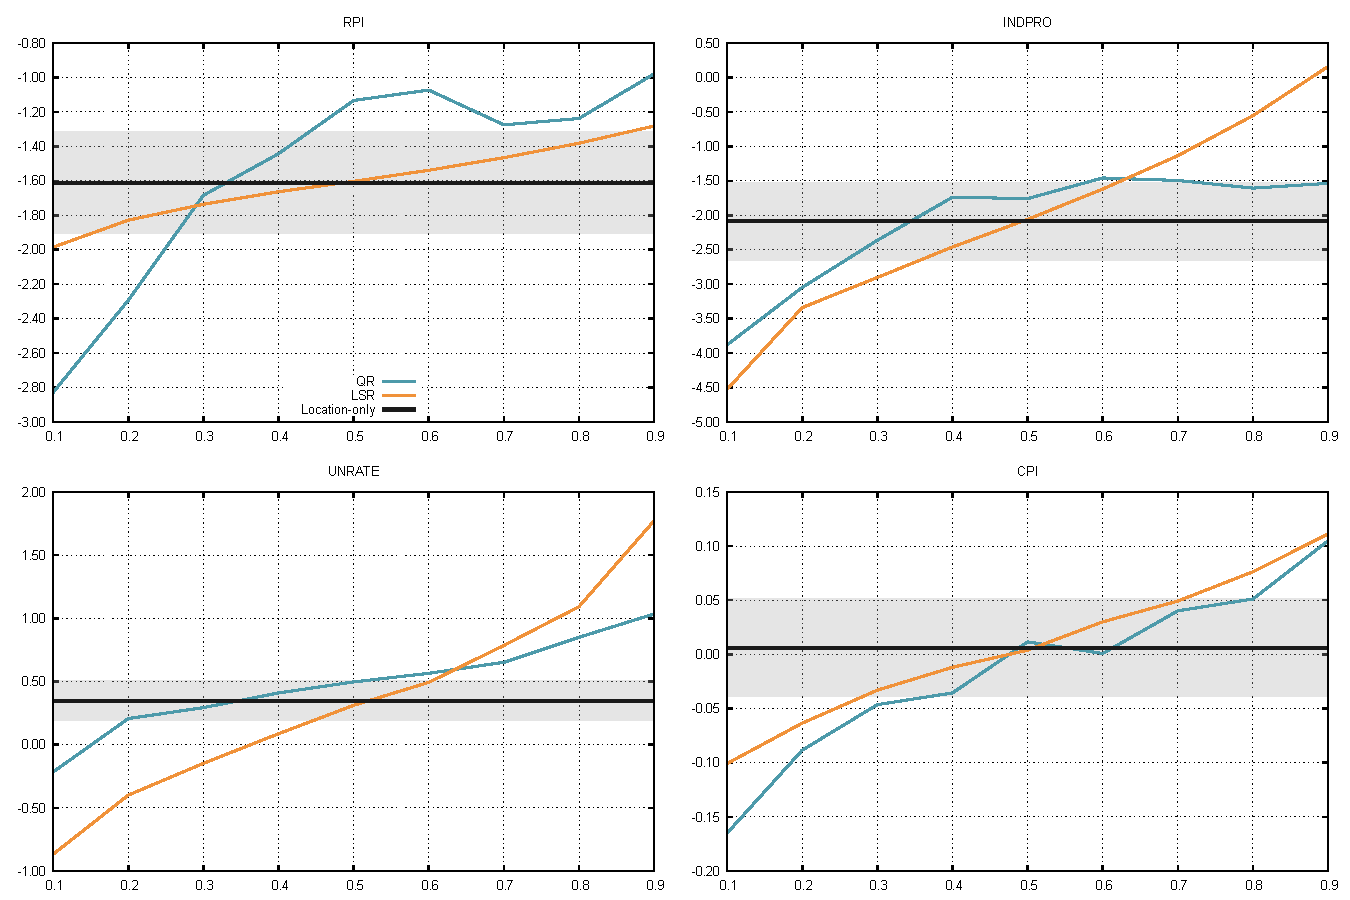
\includegraphics[width=0.95\textwidth]{figures/QIRF_plots.pdf}
	\]
	{\hspace{1em} \footnotesize This figure displays the QIRFs of selected macroeconomic variables to an increase in MUNC from its median to its 95\% quantile. The responses refer to the twelve-month forward average of Real Personal Income (RPI), Industrial Production (INDPRO), the Unemployment Rate (UNRATE), and the Consumer Price Index (CPI). The QIRFs are reported for nine equally-spaced quantiles from the 10\% to the 90\% of the distribution and are estimated using quantile regression and location–scale regression. The shaded area represents the 95\% confidence band around the location-only QIRF.
	}
\end{figure}

\begin{figure}[!htbp]
	\caption{\sc Downside Risk Factors and Macroeconomic Volatility}\label{fig:factors_and_volatility}
	\[
	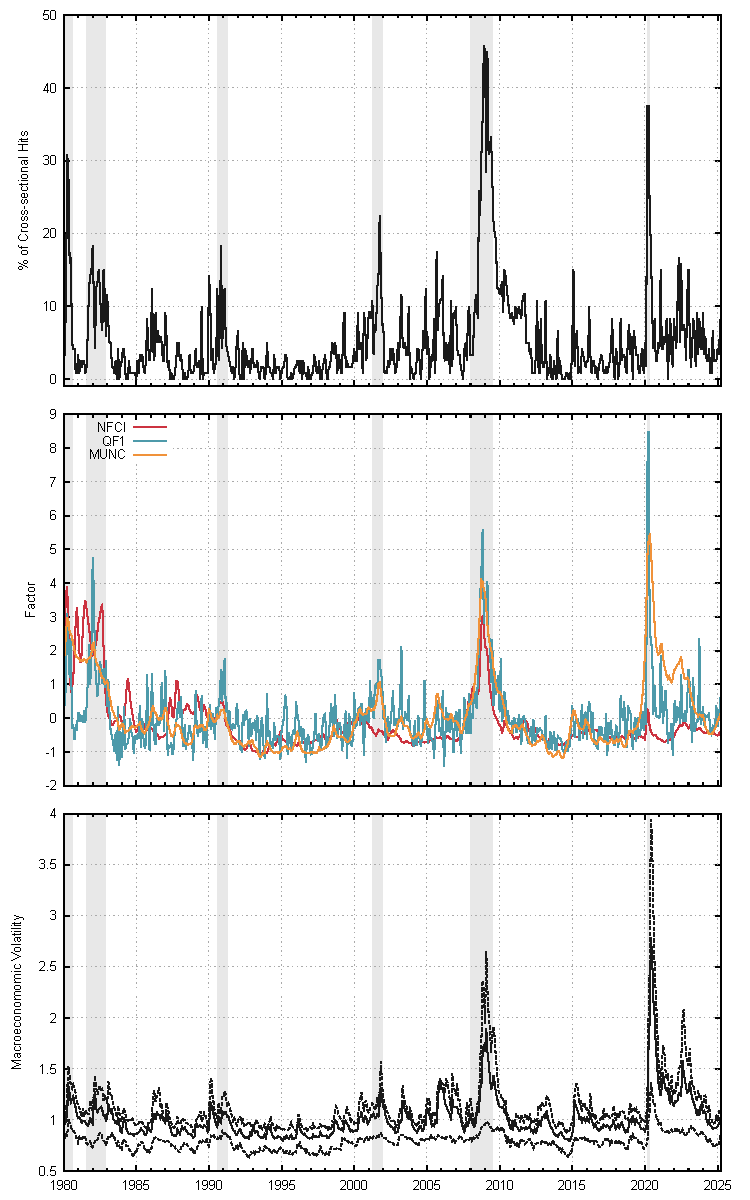
\includegraphics[width=0.95\textwidth,height=0.80\textheight,keepaspectratio]{figures/MacroVol_plots.pdf}
	\]
	{\hspace{1em} \footnotesize This figure displays the relationship between selected downside risk factors and macroeconomic volatility. The top panel reports the share of macroeconomic variables with realizations below their 5\% empirical quantile. The middle panel reports the time series of the three leading downside risk factors: NFCI, QF1, and MUNC. The bottom panel reports the cross-sectional average, along with the first and third quartiles, of the estimated macroeconomic volatility.}
\end{figure}

\end{document}
